\section{Analysis, Experiments and Results}

In this section, we will present and discuss the results obtained from the computation.

\subsection{Segmentation Results (RQ1)}

Silhouette rises from $k = 3$ to a maximum of 0.653 at $k = 8$ and drops to 0.417 at $k = 9$, and the Davies--Bouldin index reaches its minimum of 0.719 at the same $k$ (Table~\ref{tab:cluster_selection}, Fig.~\ref{fig:cluster_selection}). Every $k$ up to 8 satisfies the minimum segment size, so $k = 8$ was selected for this dataset.

\begin{table}[H]
    \centering
    \caption{Cluster-selection criteria for K-Means (silhouette, Davies--Bouldin and Cali\'nski--Harabasz on a 20,000-record sample).}
    \label{tab:cluster_selection}
    \small
    \begin{tabular}{rrrrrr}
        \toprule
        $k$ & Silhouette & Davies--Bouldin & Cali\'nski--Harabasz & Smallest segment & Largest segment (\%) \\
        \midrule
        3 & 0.550 & 1.766 & 4,405.158 & 22,566 & 73.300 \\
        4 & 0.576 & 1.429 & 4,791.651 & 14,862 & 73.400 \\
        5 & 0.605 & 1.323 & 5,443.486 & 14,716 & 73.100 \\
        6 & 0.621 & 1.132 & 6,300.054 & 5,469 & 72.800 \\
        7 & 0.643 & 0.865 & 7,873.797 & 5,429 & 72.600 \\
        8 & \textbf{0.653} & \textbf{0.719} & 8,404.810 & 4,223 & 72.500 \\
        9 & 0.417 & 0.804 & 8,626.968 & 4,205 & 58.200 \\
        10 & 0.421 & 0.844 & 8,479.447 & 3,228 & 58.000 \\
        \bottomrule
    \end{tabular}
\end{table}

\begin{figure}[H]
    \centering
    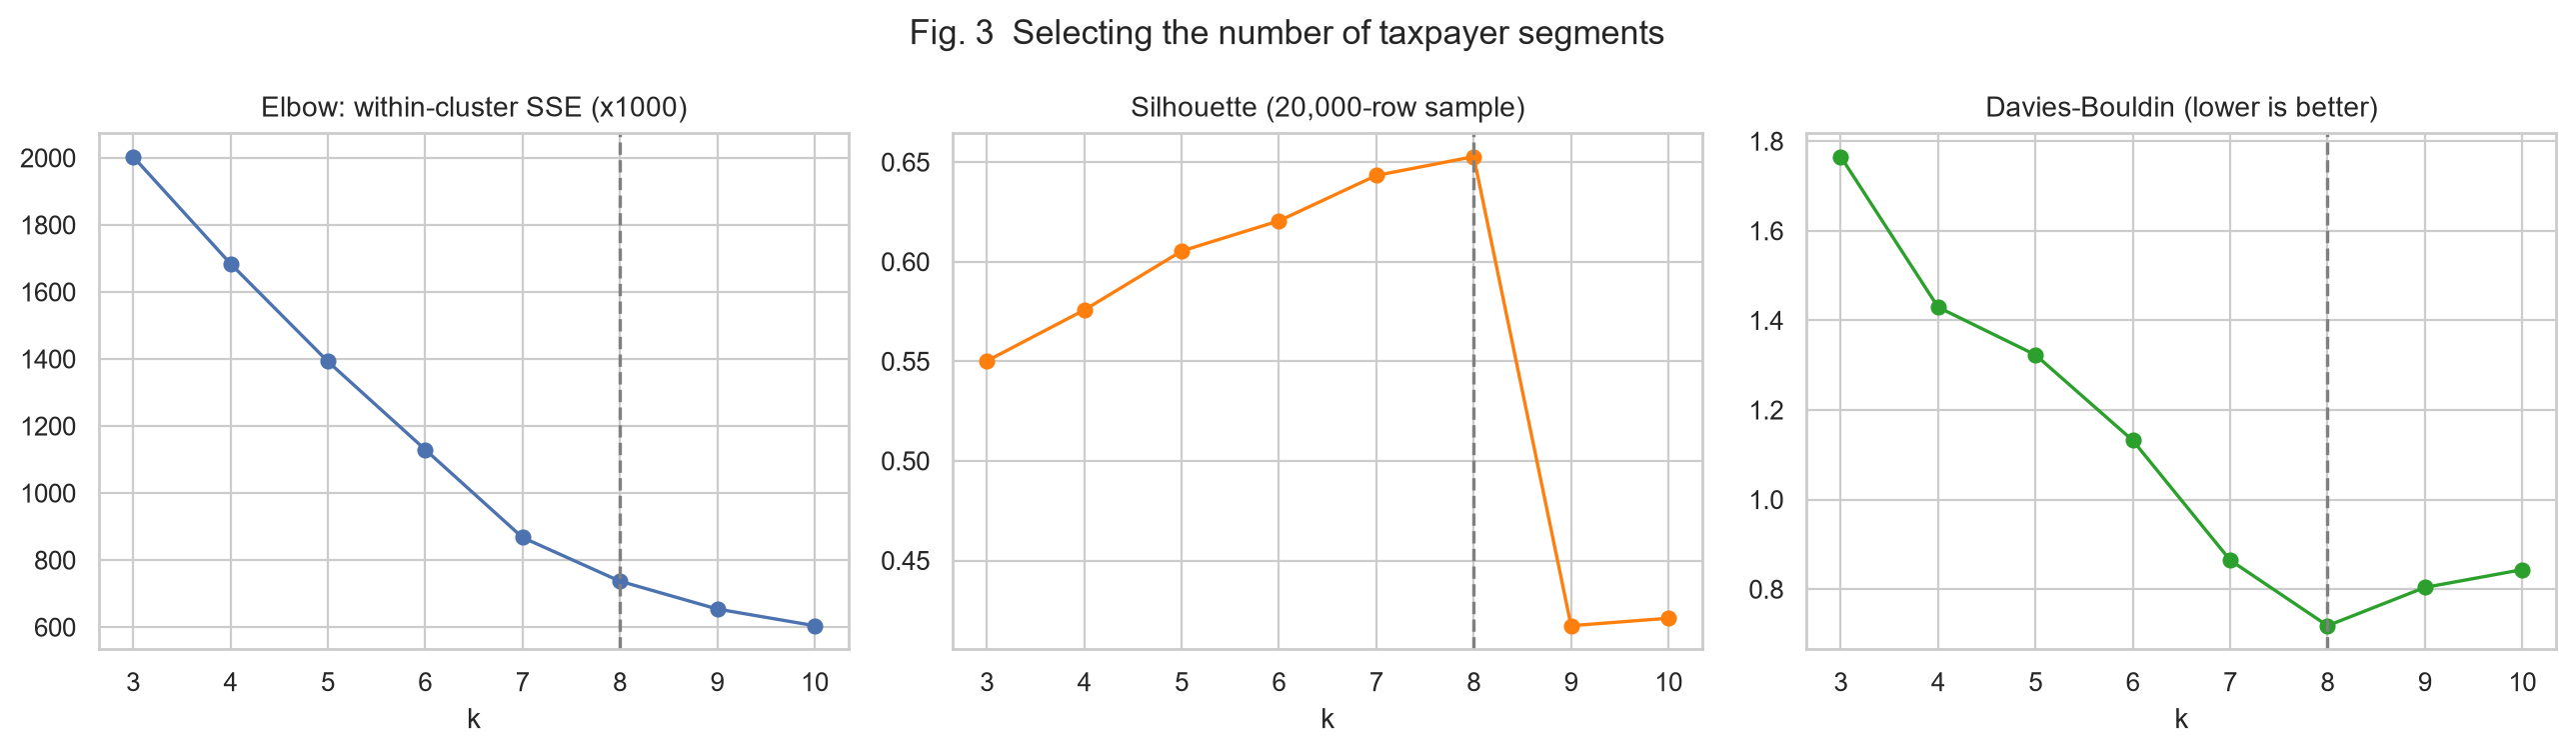
\includegraphics[width=\linewidth]{figures/fig03_cluster_selection.png}
    \caption{Selecting the number of taxpayer segments.}
    \label{fig:cluster_selection}
\end{figure}

The eight segments (Table~\ref{tab:segments}, Fig.~\ref{fig:segments}) correspond to recognisable taxpayer types without being imposed. 72.5\% of taxpayers with median income of \$67,797 belong to segment S0 and their modal age is between 30 to 34. 5.5\% of records are in Segment S1, and it is pension-dominated by 79\% population, with modal age is 70 and over and a median super balance of only \$1,722, retiree profile. Segment S2 is 88\% of business profile dominant group, which agent-lodged in 90\% of cases, median income of \$36,148. Segment S3 is 88\% investment dominant with low taxable income but a median super balance of \$141,883. Segment S5, 2.9\% of records, is rental dominant, Segment S6 4.5\% of records is trust and partnership dominant with 96.5\% agent lodgment. Majority of segment S7 reported no amount in income and deuctions with median income of \$0 and only one item being reported.

\begin{table}[H]
    \centering
    \caption{Segment profiles (medians in AUD).}
    \label{tab:segments}
    \footnotesize
    \resizebox{\textwidth}{!}{%
    \begin{tabular}{lrrrrrrrl}
        \toprule
        Segment & $n$ & Share (\%) & Median total income & Median deductions & Median super balance & Agent lodged (\%) & Modal age range & Top occupation \\
        \midrule
        S0: Wage-dominant (mid income) & 233,317 & 72.5 & 67,797 & 1,367 & 57,133 & 58.4 & 8 & Professionals \\
        S1: Pension/retirement (low income) & 17,834 & 5.5 & 23,327 & 0.0 & 1,721.5 & 44.5 & 0 & Not stated \\
        S2: Business-dominant (mid income) & 18,650 & 5.8 & 36,148 & 0.0 & 19,855.5 & 89.6 & 8 & Not stated \\
        S3: Investment-income (low income) & 18,758 & 5.8 & 16,659 & 0.0 & 141,883 & 76.9 & 0 & Not stated \\
        S4: Other-income (mid income) & 5,402 & 1.7 & 40,794.5 & 235.0 & 40,881.5 & 69.3 & 0 & Not stated \\
        S5: Rental-property (low income) & 9,266 & 2.9 & 17,606.5 & 268.5 & 72,392.5 & 86.2 & 0 & Not stated \\
        S6: Trust/partnership (mid income) & 14,440 & 4.5 & 65,278 & 184.0 & 75,413 & 96.5 & 0 & Not stated \\
        S7: No/minimal reported income & 4,223 & 1.3 & 0.0 & 0.0 & 0.0 & 36.3 & 8 & Not stated \\
        \bottomrule
    \end{tabular}}
\end{table}

\begin{figure}[H]
    \centering
    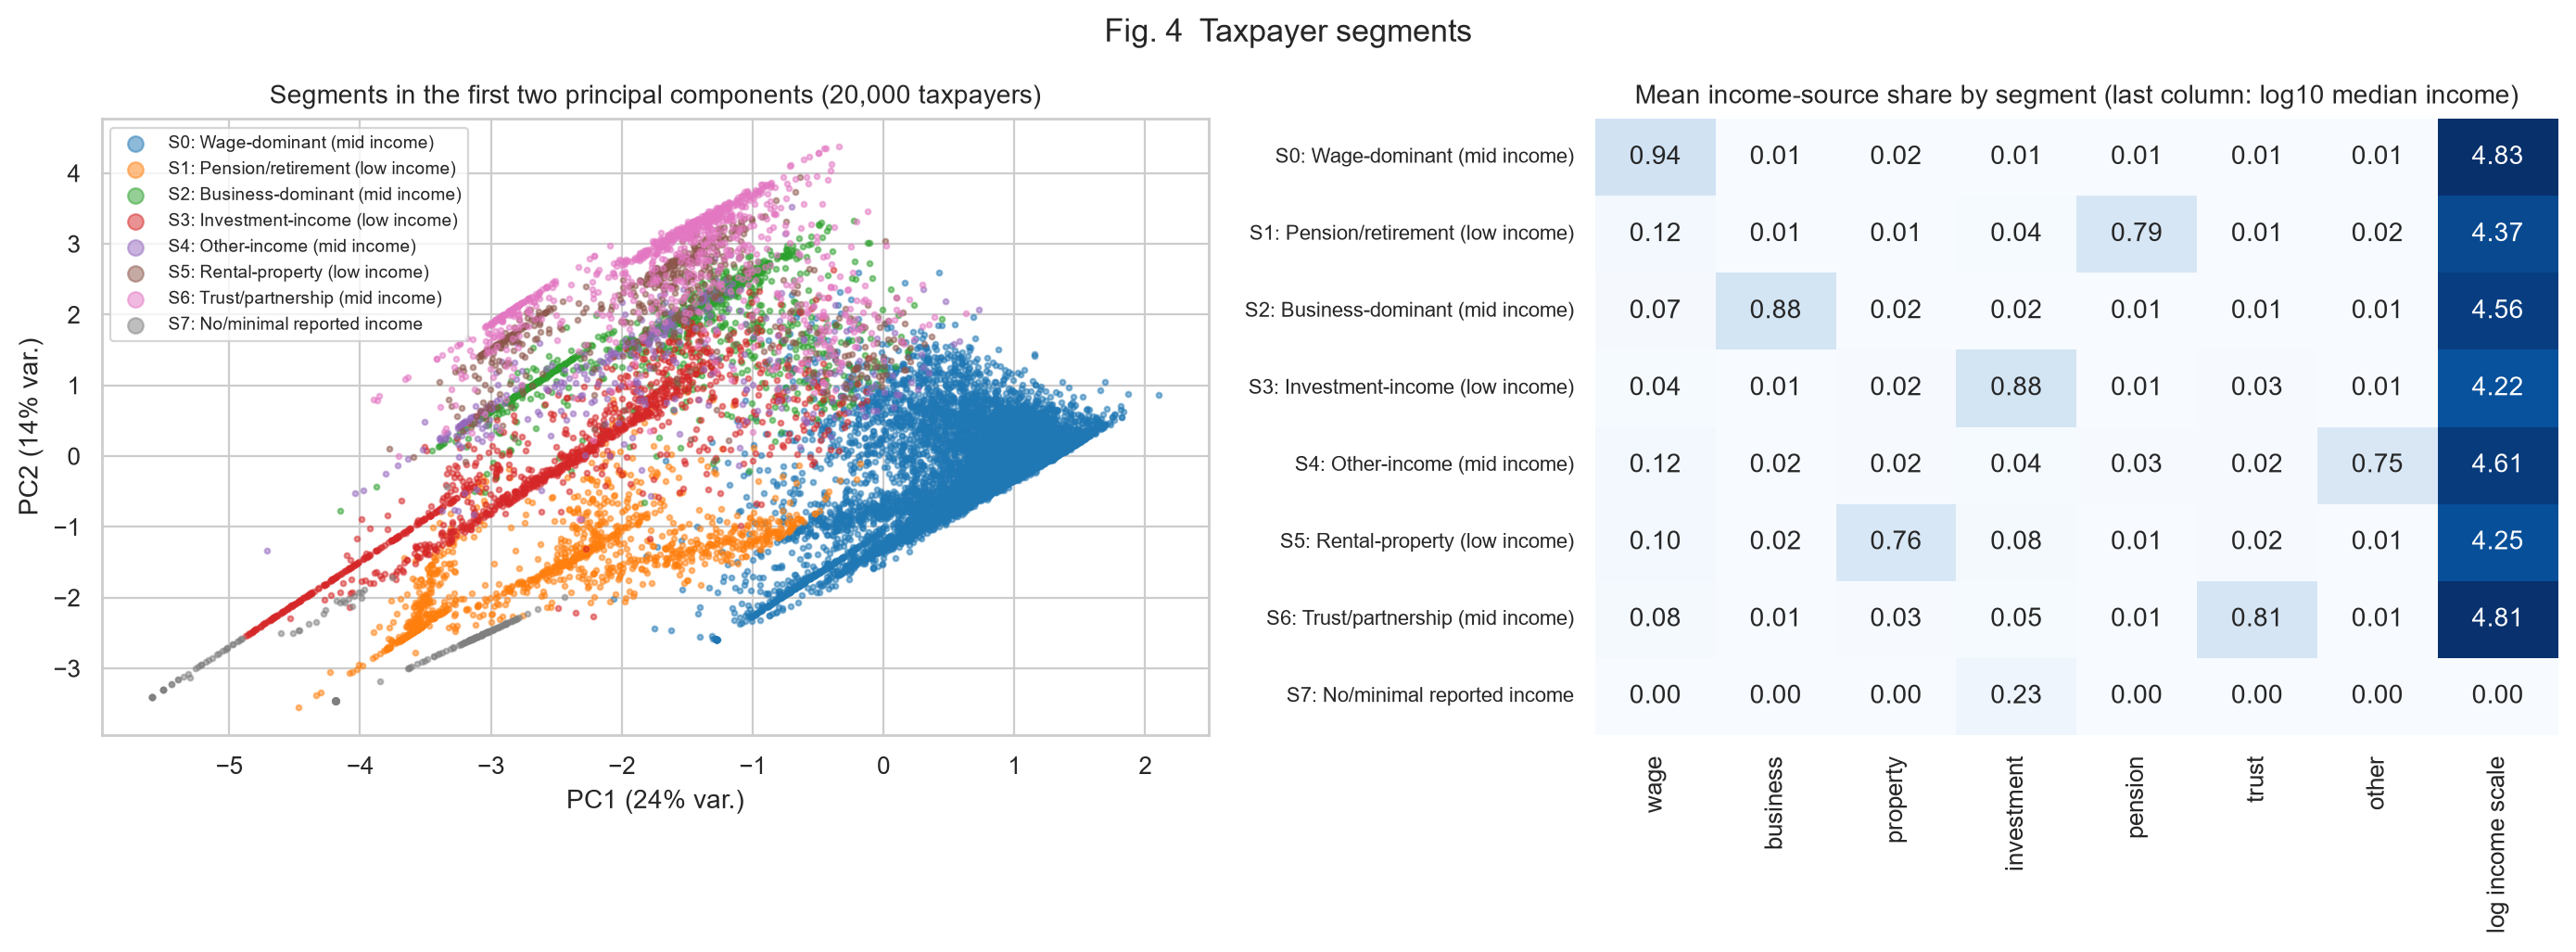
\includegraphics[width=\linewidth]{figures/fig04_segments.png}
    \caption{Taxpayer segments in the first two principal components, and mean income-source share by segment.}
    \label{fig:segments}
\end{figure}

RQ1 is answered positively that a income composition space yields well-separated and tax-interpretable peer groups, in contrast to the weak separation (silhouette 0.05--0.13) obtained on this same data when only dollar amounts were clustered not ratio.

\subsection{Unsupervised Anomaly Detection (RQ2)}

At the 2\% threshold, the design using segmentation flagged 6,442 records and the population-wide design has 6,438 records respectively. Of the segmented flags, 6,064 (94\%) were natural profiles and 378 injected records.

\begin{table}[H]
    \centering
    \caption{Within-segment anomaly-score thresholds and number flagged at each contamination level.}
    \label{tab:thresholds}
    \footnotesize
    \resizebox{\textwidth}{!}{%
    \begin{tabular}{lrrrrrr}
        \toprule
        Segment & $n$ & Threshold 1\% & Threshold 2\% & Threshold 5\% & Threshold 10\% & Flagged at 2\% \\
        \midrule
        S0: Wage-dominant (mid income) & 233,317 & 0.5616 & 0.5332 & 0.4915 & 0.4567 & 4,667 \\
        S1: Pension/retirement (low income) & 17,834 & 0.5603 & 0.5294 & 0.4835 & 0.4472 & 357 \\
        S2: Business-dominant (mid income) & 18,650 & 0.5768 & 0.5425 & 0.4960 & 0.4553 & 373 \\
        S3: Investment-income (low income) & 18,758 & 0.5628 & 0.5449 & 0.5102 & 0.4781 & 376 \\
        S4: Other-income (mid income) & 5,402 & 0.5470 & 0.5286 & 0.4921 & 0.4641 & 109 \\
        S5: Rental-property (low income) & 9,266 & 0.5509 & 0.5263 & 0.4929 & 0.4615 & 186 \\
        S6: Trust/partnership (mid income) & 14,440 & 0.5459 & 0.5234 & 0.4892 & 0.4580 & 289 \\
        S7: No/minimal reported income & 4,223 & 0.5761 & 0.5394 & 0.4854 & 0.4410 & 85 \\
        \bottomrule
    \end{tabular}}
\end{table}

\begin{figure}[H]
    \centering
    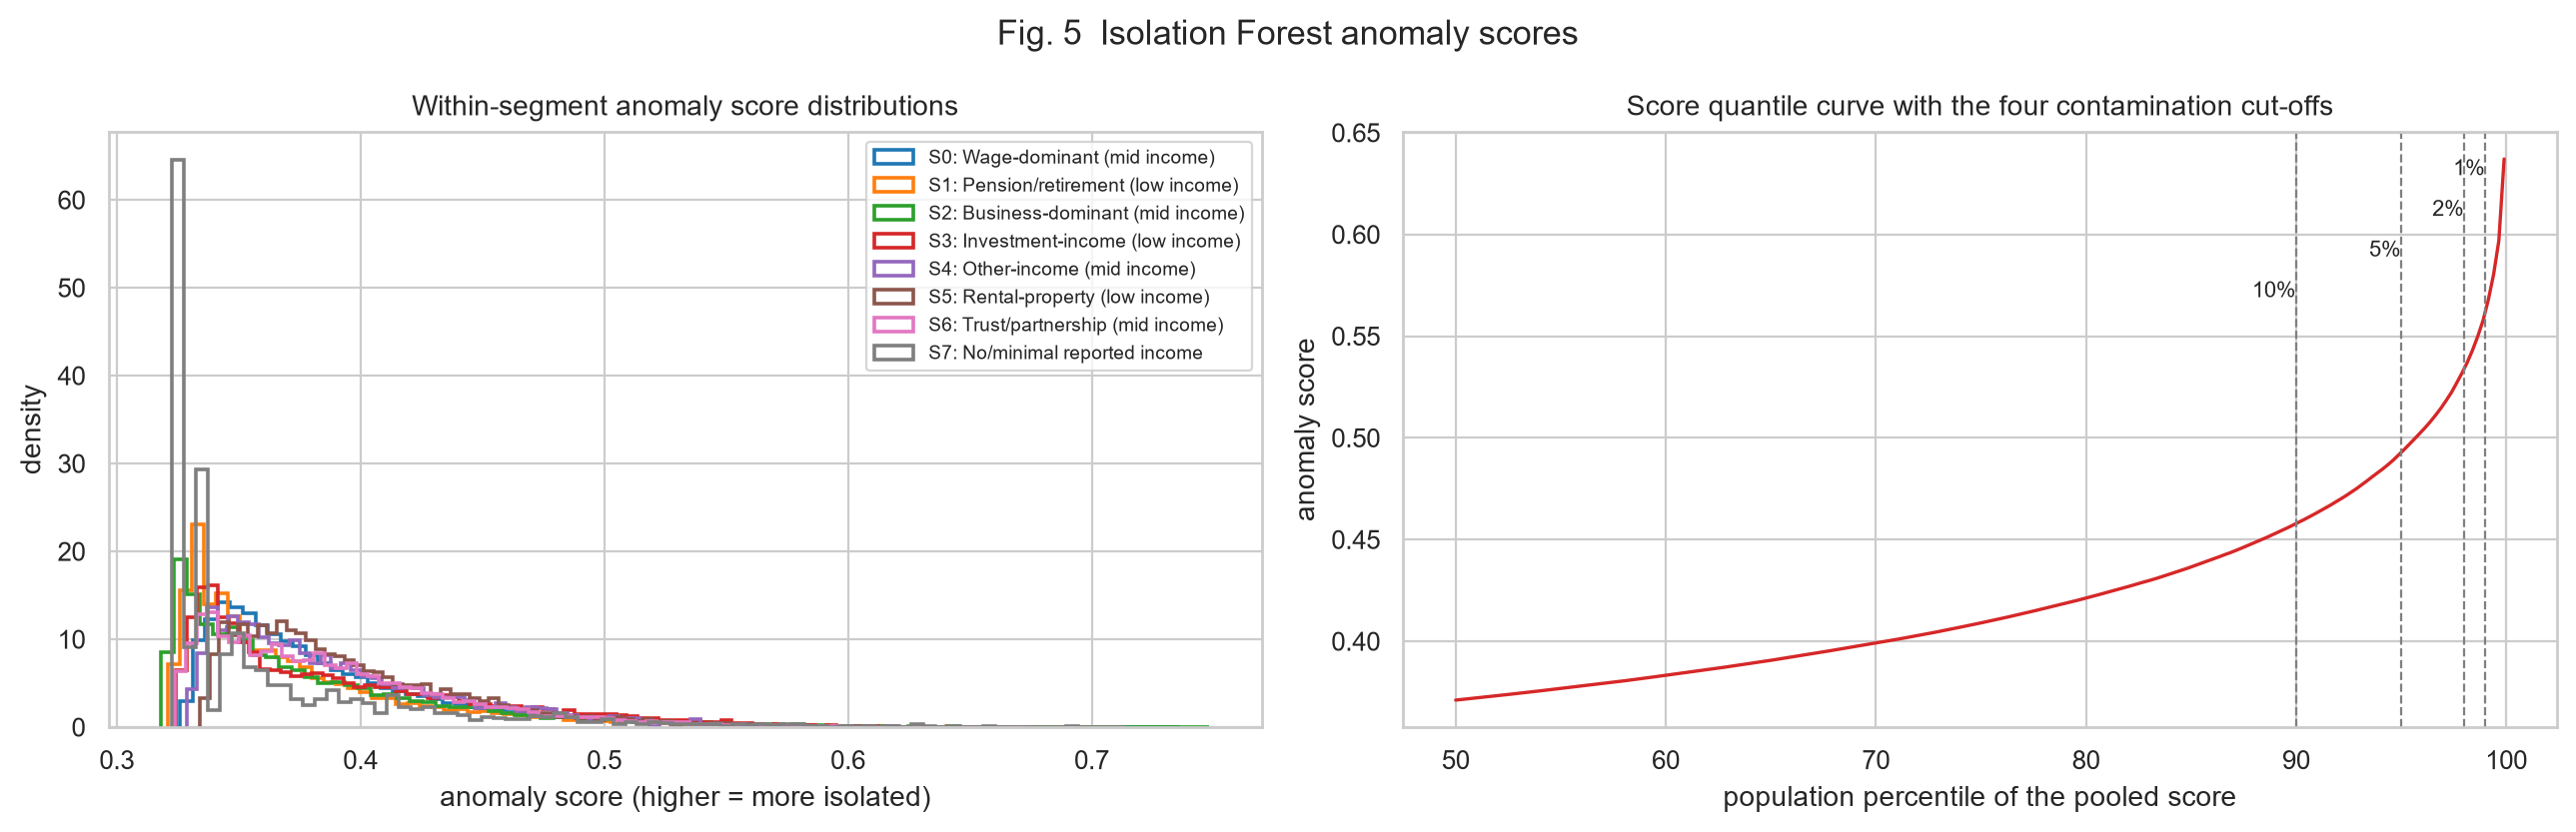
\includegraphics[width=\linewidth]{figures/fig05_anomaly_scores.png}
    \caption{Isolation Forest anomaly scores within segment distribution and the pooled quantile curve with the cut-offs.}
    \label{fig:anomaly_scores}
\end{figure}

Raising the threshold from 1\% to 10\% raised recall of injected anomalies from 6.8\% to 44.7\% in segmented anomaly and from 8.3\% to 48.8\% in population-wide anomaly, while precision against the injected labels fell from about 7\% to 4.5\% as shown below (Table~\ref{tab:sweep}).

\begin{table}[H]
    \centering
    \caption{Contamination results per segment and population.}
    \label{tab:sweep}
    \footnotesize
    \resizebox{\textwidth}{!}{%
    \begin{tabular}{rlrrrrr}
        \toprule
        Contamination & Design & Flagged & Injected recall & Injected precision & Injected F1 & Natural flags \\
        \midrule
        0.010 & segmented & 3,224 & 0.068 & 0.068 & 0.068 & 3,006 \\
        0.010 & population-wide & 3,219 & 0.083 & 0.083 & 0.083 & 2,953 \\
        0.020 & segmented & 6,442 & 0.117 & 0.059 & 0.078 & 6,064 \\
        0.020 & population-wide & 6,438 & 0.141 & 0.070 & 0.094 & 5,985 \\
        0.050 & segmented & 16,098 & 0.251 & 0.050 & 0.084 & 15,289 \\
        0.050 & population-wide & 16,095 & 0.277 & 0.055 & 0.092 & 15,205 \\
        0.100 & segmented & 32,192 & 0.447 & 0.045 & 0.081 & 30,754 \\
        0.100 & population-wide & 32,189 & 0.488 & 0.049 & 0.089 & 30,619 \\
        \bottomrule
    \end{tabular}}
\end{table}

The designs agree on 3,909 taxpayers with Jaccard score 0.436 and Spearman correlation of scores 0.795, so it means segmentation changed more than half of the list. The population-wide anomaly concentrated in the small non-wage segments where 8.2\% of investment-income taxpayers, 6.2\% of landlords, 4.8\% of other-income and 4.3\% of trust-distribution taxpayers (Fig.~\ref{fig:seg_vs_global}). These taxpayers were flagged because their type of return compared with all population and majority of population has wage related income. Whereas segmented design equalises this burden at 2\% of every peer group. On the pre-specified benchmark, however, segmentation did not improve sensitivity: recall was slightly lower (11.7\% versus 14.1\%), and by type the segmented forest was better only for work-related-expense inflation (9.6\% versus 6.2\%), while the population-wide forest recovered more business-expense (21.4\% versus 15.2\%) and rental-deduction anomalies (31.5\% versus 23.1\%). The taxable-income identity violation was nearly invisible to both (1.4\% and 2.0\%) because it perturbs one feature among 56, and isolation rewards records that are extreme on many. Income confounding was not reduced either: 46.9\% of segmented and 46.1\% of population-wide flags fell in the top income decile, and the score--income rank correlation rose from 0.14 to 0.25, because within the large wage segment scale remains the dominant source of rarity (Table~\ref{tab:confounding}).

\begin{table}[H]
    \centering
    \caption{Overlap and income confounding of the two designs at the 2\% budget.}
    \label{tab:confounding}
    \small
    \begin{tabular}{lrr}
        \toprule
        & Segmented & Population-wide \\
        \midrule
        Flagged & 6,442 & 6,438 \\
        Median income of flagged (AUD) & 139,872 & 135,241.5 \\
        Income multiple of population median & 2.408 & 2.328 \\
        Flagged in top income decile (\%) & 46.880 & 46.070 \\
        Flagged below median income (\%) & 17.665 & 23.035 \\
        Spearman correlation, score vs.\ income & 0.250 & 0.140 \\
        \bottomrule
    \end{tabular}
\end{table}

\begin{figure}[H]
    \centering
    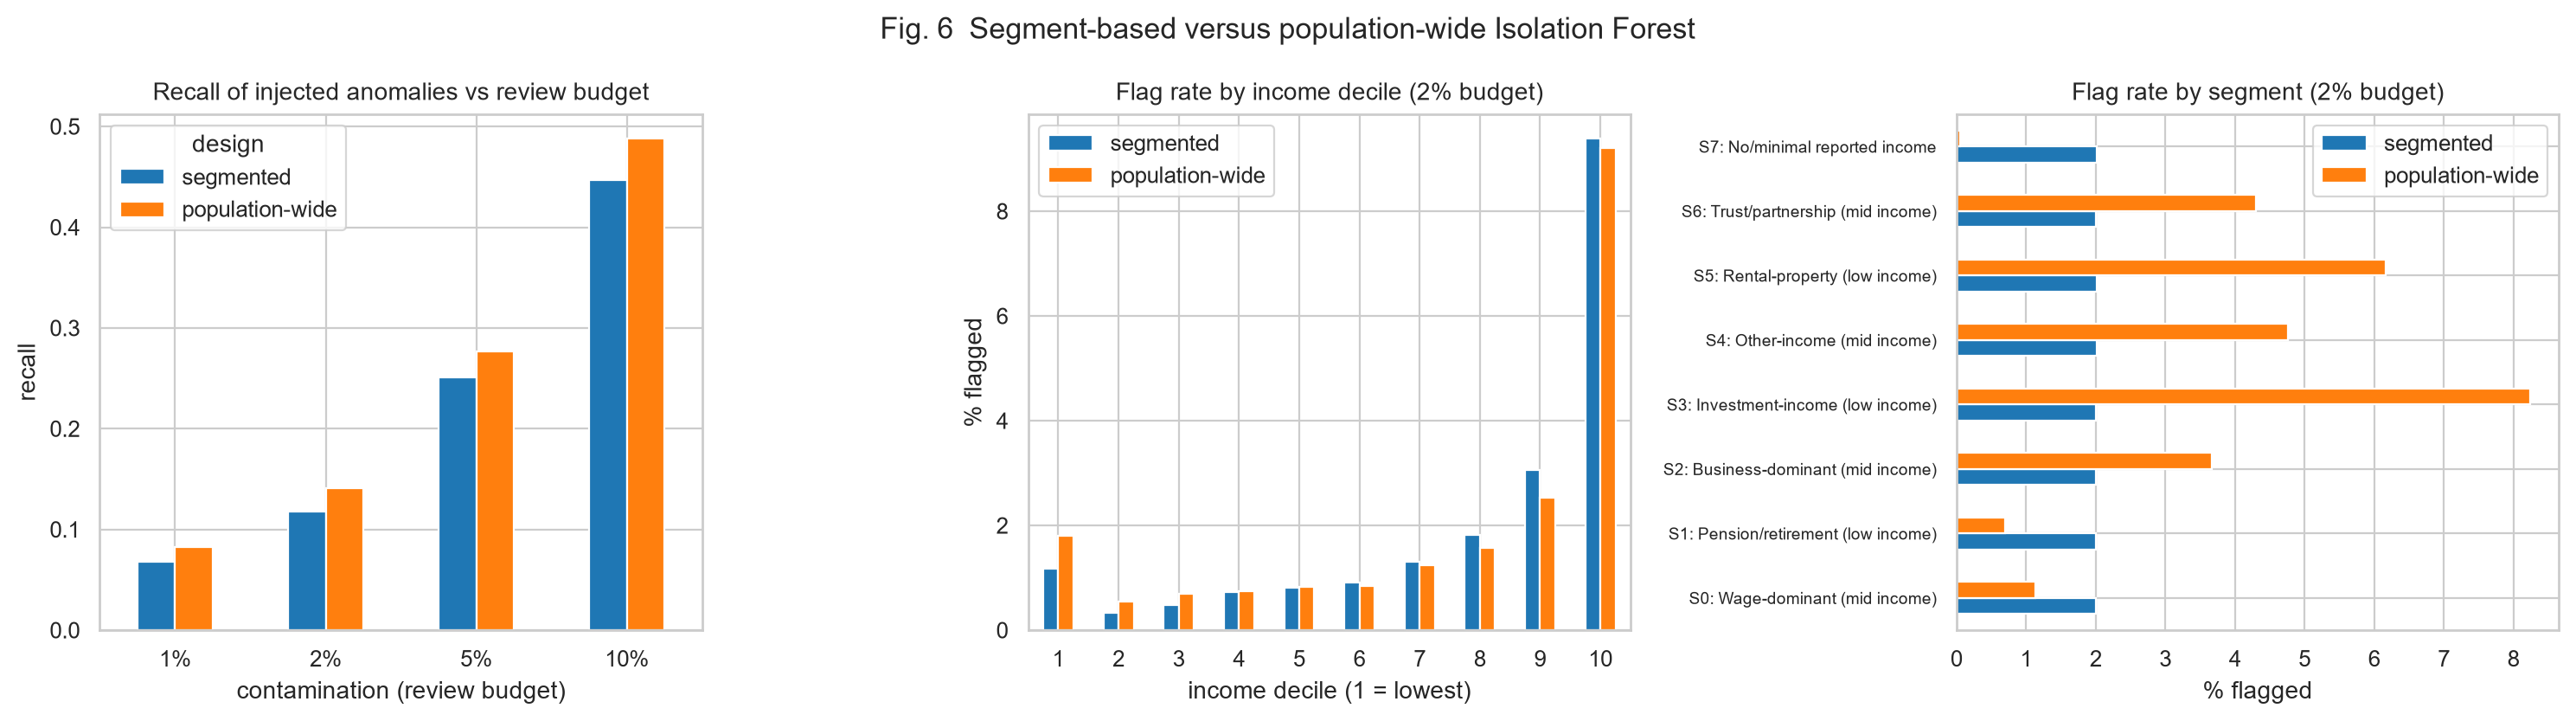
\includegraphics[width=\linewidth]{figures/fig06_segmented_vs_global.png}
    \caption{Segment-based versus population-wide Isolation Forest: recall of injected anomalies by budget, flag rate by income decile and by segment.}
    \label{fig:seg_vs_global}
\end{figure}

Repeating both designs on the twelve behavioural ratios alone changed the picture completely (Tables~\ref{tab:ablation} and \ref{tab:recall_by_type}). At the same 2\% budget recall of injected anomalies rose from 11.7\% to 39.6\% (segmented) and from 14.1\% to 41.7\% (population-wide), precision from 6--7\% to 20--21\%, and PR-AUC against the injected labels from 0.04--0.05 to 0.22. The share of flags in the top income decile fell from 47\% to 15--16\%, and the score--income correlation fell to 0.12 (segmented) and to zero (population-wide). Anomaly score for taxpayers with investment deductions without having investment income rose from 9\% to 98\%, and business expense and rental deduction inflation to 38--49\%. Work related expense inflation remained because a 25--45\% claim is not extreme relative to the whole ratio distribution, and the identity violation remained undetected. Only 2,370 records were flagged by both the primary and the ratio only methods, so the choice of feature changes the anomaly list as much as the choice of reference population.

\begin{table}[H]
    \centering
    \caption{Ablation: design $\times$ feature space at the 2\% budget.}
    \label{tab:ablation}
    \footnotesize
    \resizebox{\textwidth}{!}{%
    \begin{tabular}{llrrrrrr}
        \toprule
        Feature space & Design & Flagged & Injected recall & Injected precision & PR-AUC vs.\ injected & Flagged in top income decile (\%) & Spearman score vs.\ income \\
        \midrule
        amounts + ratios (primary) & segmented & 6,442 & 0.117 & 0.059 & 0.044 & 46.880 & 0.250 \\
        amounts + ratios (primary) & population-wide & 6,438 & 0.141 & 0.070 & 0.051 & 46.070 & 0.140 \\
        ratios only & segmented & 6,442 & 0.396 & 0.198 & 0.216 & 15.554 & 0.119 \\
        ratios only & population-wide & 6,438 & 0.417 & 0.208 & 0.225 & 14.585 & $-0.007$ \\
        \bottomrule
    \end{tabular}}
\end{table}

\begin{table}[H]
    \centering
    \caption{Recall of each injected mechanism by feature space and design (2\% budget).}
    \label{tab:recall_by_type}
    \footnotesize
    \begin{tabular}{lrrrr}
        \toprule
        & \multicolumn{2}{c}{amounts + ratios (primary)} & \multicolumn{2}{c}{ratios only} \\
        \cmidrule(lr){2-3} \cmidrule(lr){4-5}
        Anomaly type & segmented & population-wide & segmented & population-wide \\
        \midrule
        A1 WRE inflation & 0.096 & 0.062 & 0.214 & 0.115 \\
        A2 Business expense & 0.152 & 0.214 & 0.376 & 0.486 \\
        A3 Rental deduction & 0.231 & 0.315 & 0.390 & 0.470 \\
        A4 Taxable identity & 0.014 & 0.020 & 0.026 & 0.023 \\
        A5 Investment deduction, no income & 0.093 & 0.092 & 0.975 & 0.991 \\
        \bottomrule
    \end{tabular}
\end{table}

The answer to RQ2 is therefore confirmed. Segmentation changes which taxpayers is being reviewed and removes the over representation of rare taxpayer types. Segmentation alone did not make Isolation Forest sensitive at identifying unusual reporting behaviour as the model remained strongly influenced by raw dollar amounts as well. Ratio-based features were needed to remove the effect of scale. Once these behavioural ratios were included, segmentation produced only a small further improvement in anomaly sensitivity.

\subsection{Supervised Learning Results (RQ3)}

On the set of 96,567 taxpayers (966 injected) the Random Forest achieved precision for 89\%, recall for 94\% at threshold 0.5, with 109 false positives and 56 false negatives (Table~\ref{tab:supervised}, Fig.~\ref{fig:supervised}). Gradient boosting have precision at 72\% and recall at 98\% and trained sixteen times faster. Five-fold cross-validation confirmed the ranking (F1 $0.920 \pm 0.009$ versus $0.856 \pm 0.028$; PR-AUC 0.970 versus 0.974). Accuracy was 99.8\% for both.

\begin{table}[H]
    \centering
    \caption{Supervised classification of injected anomalies on the hold-out set.}
    \label{tab:supervised}
    \footnotesize
    \resizebox{\textwidth}{!}{%
    \begin{tabular}{llrrrrrrrrrr}
        \toprule
        Model & Threshold & Accuracy & Precision & Recall & F1 & ROC-AUC & PR-AUC & TP & FP & FN & TN \\
        \midrule
        Random Forest & 0.50 & 0.998 & 0.893 & 0.942 & 0.917 & 1.000 & 0.975 & 910 & 109 & 56 & 95,492 \\
        Random Forest & top 2\% budget & 0.990 & 0.499 & 0.998 & 0.665 & 1.000 & 0.975 & 964 & 967 & 2 & 94,634 \\
        Hist.\ Gradient Boosting & 0.50 & 0.996 & 0.727 & 0.980 & 0.835 & 0.997 & 0.968 & 947 & 356 & 19 & 95,245 \\
        Hist.\ Gradient Boosting & top 2\% budget & 0.990 & 0.496 & 0.992 & 0.661 & 0.997 & 0.968 & 958 & 973 & 8 & 94,628 \\
        \bottomrule
    \end{tabular}}
\end{table}

\begin{figure}[H]
    \centering
    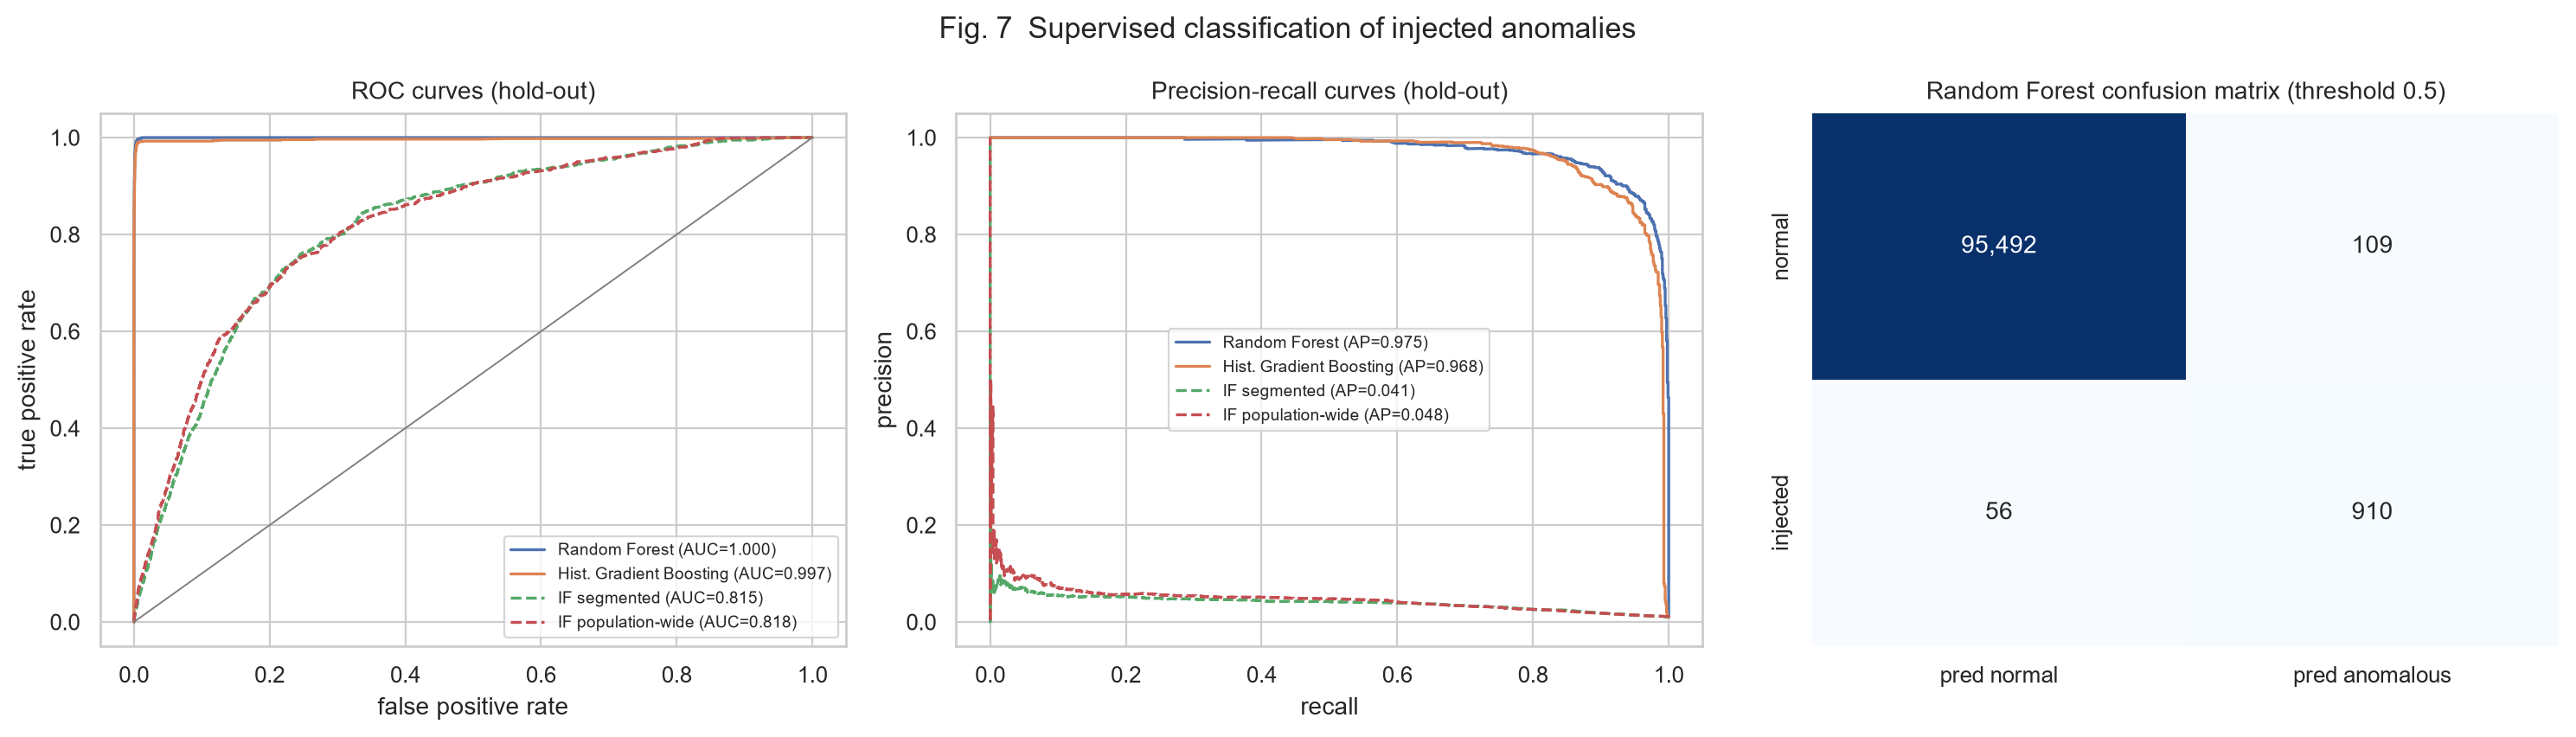
\includegraphics[width=\linewidth]{figures/fig07_supervised_evaluation.png}
    \caption{Supervised classification: ROC and precision--recall curves for both classifiers and both forests, and the Random Forest confusion matrix.}
    \label{fig:supervised}
\end{figure}

Compared on identical hold-out rows and the same 2\% budget (Table~\ref{tab:sup_vs_unsup}) the supervised models recovered almost every injected record (recall 0.998 and 0.992, precision 0.50) whereas the two primary forests recovered 10.7\% and 12.7\% (PR-AUC 0.04--0.05). This gap must not be read as the supervised model being a better fraud detector: it was shown labelled examples of five mechanisms and learned them, while the forests ranked general unusualness with no labels. The two paradigms answer different questions, which their disagreement on natural profiles makes explicit: of the 1,820 unmodified taxpayers flagged by the segmented forest in the hold-out set, the Random Forest labelled 0.6\% as anomalous. Operationally, a supervised model generalises only to mechanisms represented in its labels; an unsupervised model retains the ability to surface patterns nobody has labelled.

\begin{table}[H]
    \centering
    \caption{Supervised versus unsupervised detection of injected anomalies on identical hold-out rows and review budget.}
    \label{tab:sup_vs_unsup}
    \footnotesize
    \begin{tabular}{lrrrrrr}
        \toprule
        Method & Flagged & Precision & Recall & F1 & ROC-AUC & PR-AUC \\
        \midrule
        Isolation Forest, segmented (2\%) & 1,923 & 0.054 & 0.107 & 0.071 & 0.815 & 0.041 \\
        Isolation Forest, population-wide (2\%) & 1,926 & 0.064 & 0.127 & 0.085 & 0.818 & 0.048 \\
        Random Forest (top 2\% budget) & 1,931 & 0.499 & 0.998 & 0.665 & 1.000 & 0.975 \\
        Hist.\ Gradient Boosting (top 2\% budget) & 1,931 & 0.496 & 0.992 & 0.661 & 0.997 & 0.968 \\
        \bottomrule
    \end{tabular}
\end{table}

\subsection{SHAP Results (RQ4)}

The Random Forest reproduced the K-Means labels with 99.7\% hold-out accuracy, so its explanations can be read as explanations of the segmentation. Wage share was the most influential feature with mean SHAP score of 0.064, followed by business, investment, pension and trust shares (Fig.~\ref{fig:shap_segmentation}). Each segment is explained mainly by its own dominant share, but the no-income segment is the only one explained chiefly by scale. A taxpayer is placed in a segment because of what kind of income they report, not how much.

\begin{figure}[H]
    \centering
    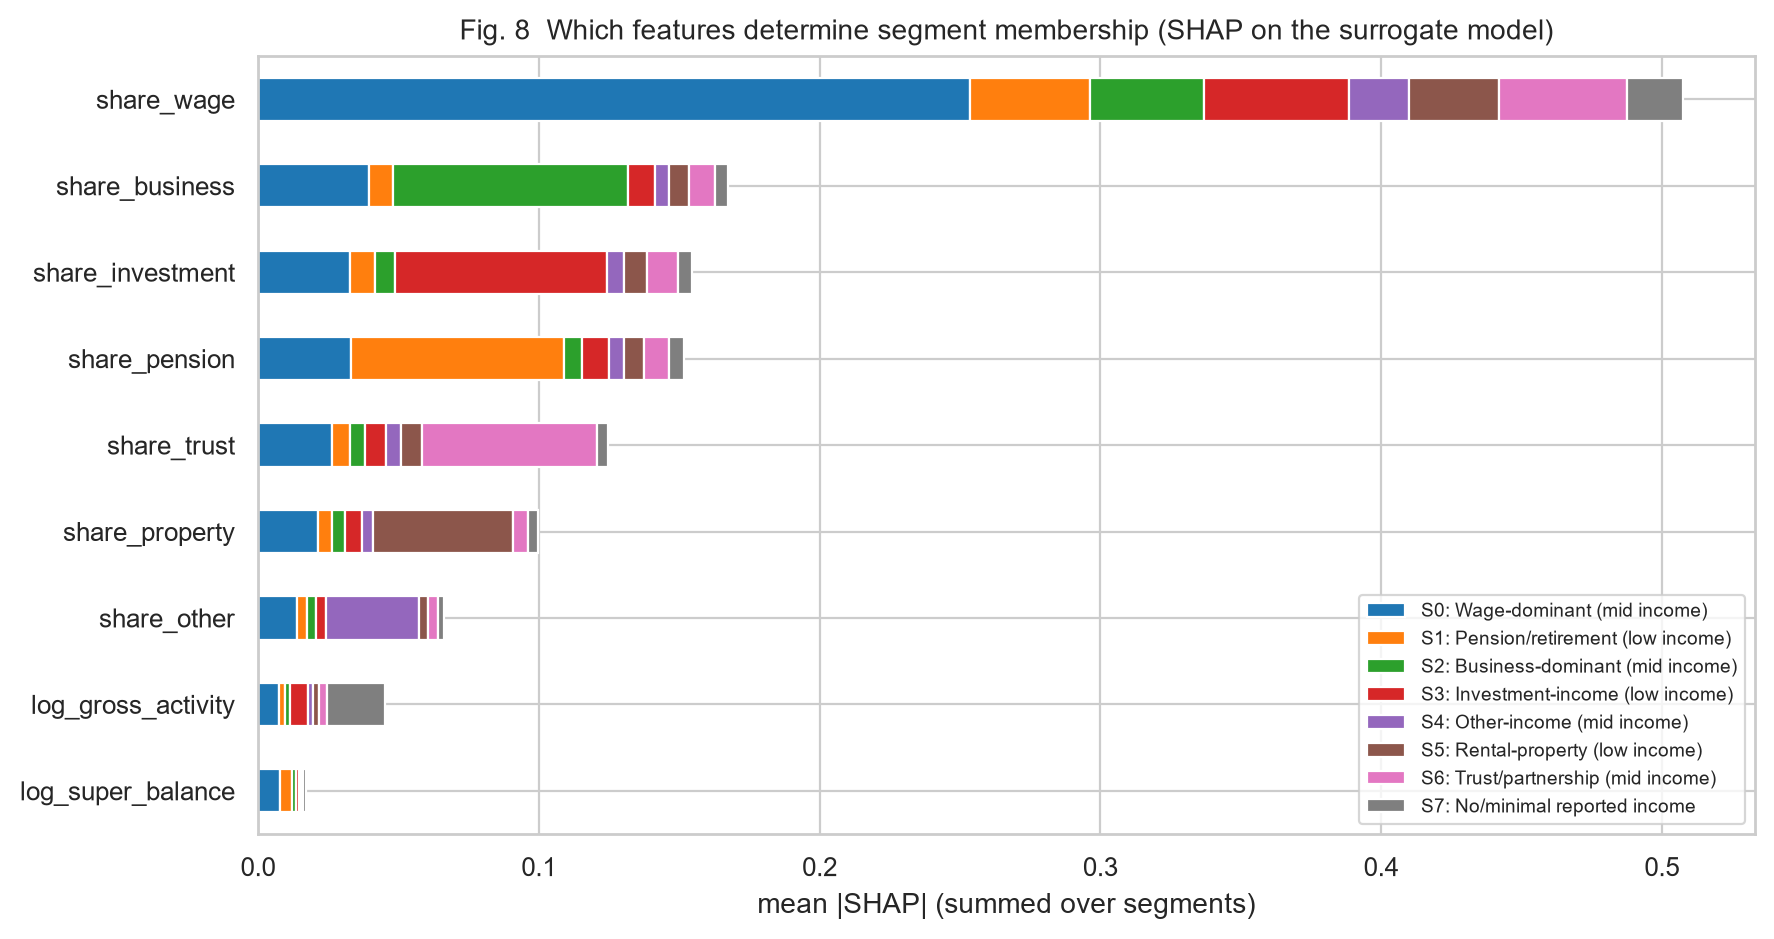
\includegraphics[width=0.85\linewidth]{figures/fig08_shap_segmentation.png}
    \caption{SHAP on the surrogate model: which features determine segment membership, stacked by segment.}
    \label{fig:shap_segmentation}
\end{figure}

The validity check passed in every segment: the sum of SHAP values tracked the forest's own score with Spearman correlation 1.000. Pooled over the segment forests (Fig.~\ref{fig:shap_if_global}, Table~\ref{tab:shap_if}) the most influential features were gross rent (mean $|$SHAP$|$ 0.196), other foreign income (0.189), total capital gains (0.189), personal superannuation contributions (0.183), gifts (0.166) and net capital gains (0.165); the deduction-to-income ratio ranks thirteenth (0.122) but has the strongest monotone relationship between value and contribution (Spearman 0.92). Every top feature contributes in the same direction: high values push toward ``anomalous'', low values are neutral. The primary forests therefore flag taxpayers who report unusual amounts of items most peers do not report at all, and secondarily taxpayers whose deductions are large relative to income; this is the mechanism behind the income confounding and the ablation result above.

\begin{table}[H]
    \centering
    \caption{Global SHAP importance of the segment Isolation Forests (pooled, top 15).}
    \label{tab:shap_if}
    \footnotesize
    \resizebox{\textwidth}{!}{%
    \begin{tabular}{lrrrr}
        \toprule
        Feature & Mean $|$SHAP$|$ & Mean contribution (flagged) & Mean contribution (unflagged) & Corr.\ value vs.\ contribution \\
        \midrule
        Gross\_rent\_amt & 0.196 & 0.281 & $-0.002$ & 0.732 \\
        Other\_foreign\_inc\_amt & 0.189 & 0.270 & $-0.007$ & 0.765 \\
        Tot\_CY\_CG\_amt & 0.189 & 0.291 & $-0.002$ & 0.807 \\
        Spr\_Prsnl\_Contr & 0.182 & 0.202 & 0.005 & 0.783 \\
        Gift\_amt & 0.166 & 0.179 & 0.007 & 0.827 \\
        Net\_CG\_amt & 0.165 & 0.238 & $-0.003$ & 0.758 \\
        Asbl\_forgn\_source\_incm\_amt & 0.155 & 0.216 & $-0.000$ & 0.787 \\
        Unfranked\_Div\_amt & 0.153 & 0.182 & $-0.003$ & 0.756 \\
        Rent\_int\_ded\_amt & 0.141 & 0.195 & $-0.005$ & 0.749 \\
        Spr\_Emplr\_Contr & 0.131 & 0.112 & $-0.006$ & 0.733 \\
        Div\_Ded\_amt & 0.124 & 0.186 & $-0.003$ & 0.566 \\
        Non\_emp\_spr\_amt & 0.123 & 0.166 & $-0.006$ & 0.685 \\
        deduction\_to\_income\_ratio & 0.122 & 0.202 & 0.002 & 0.919 \\
        Rent\_cap\_wks\_amt & 0.122 & 0.183 & $-0.000$ & 0.741 \\
        WRE\_other\_amt & 0.119 & 0.127 & $-0.004$ & 0.638 \\
        \bottomrule
    \end{tabular}}
\end{table}

\begin{figure}[H]
    \centering
    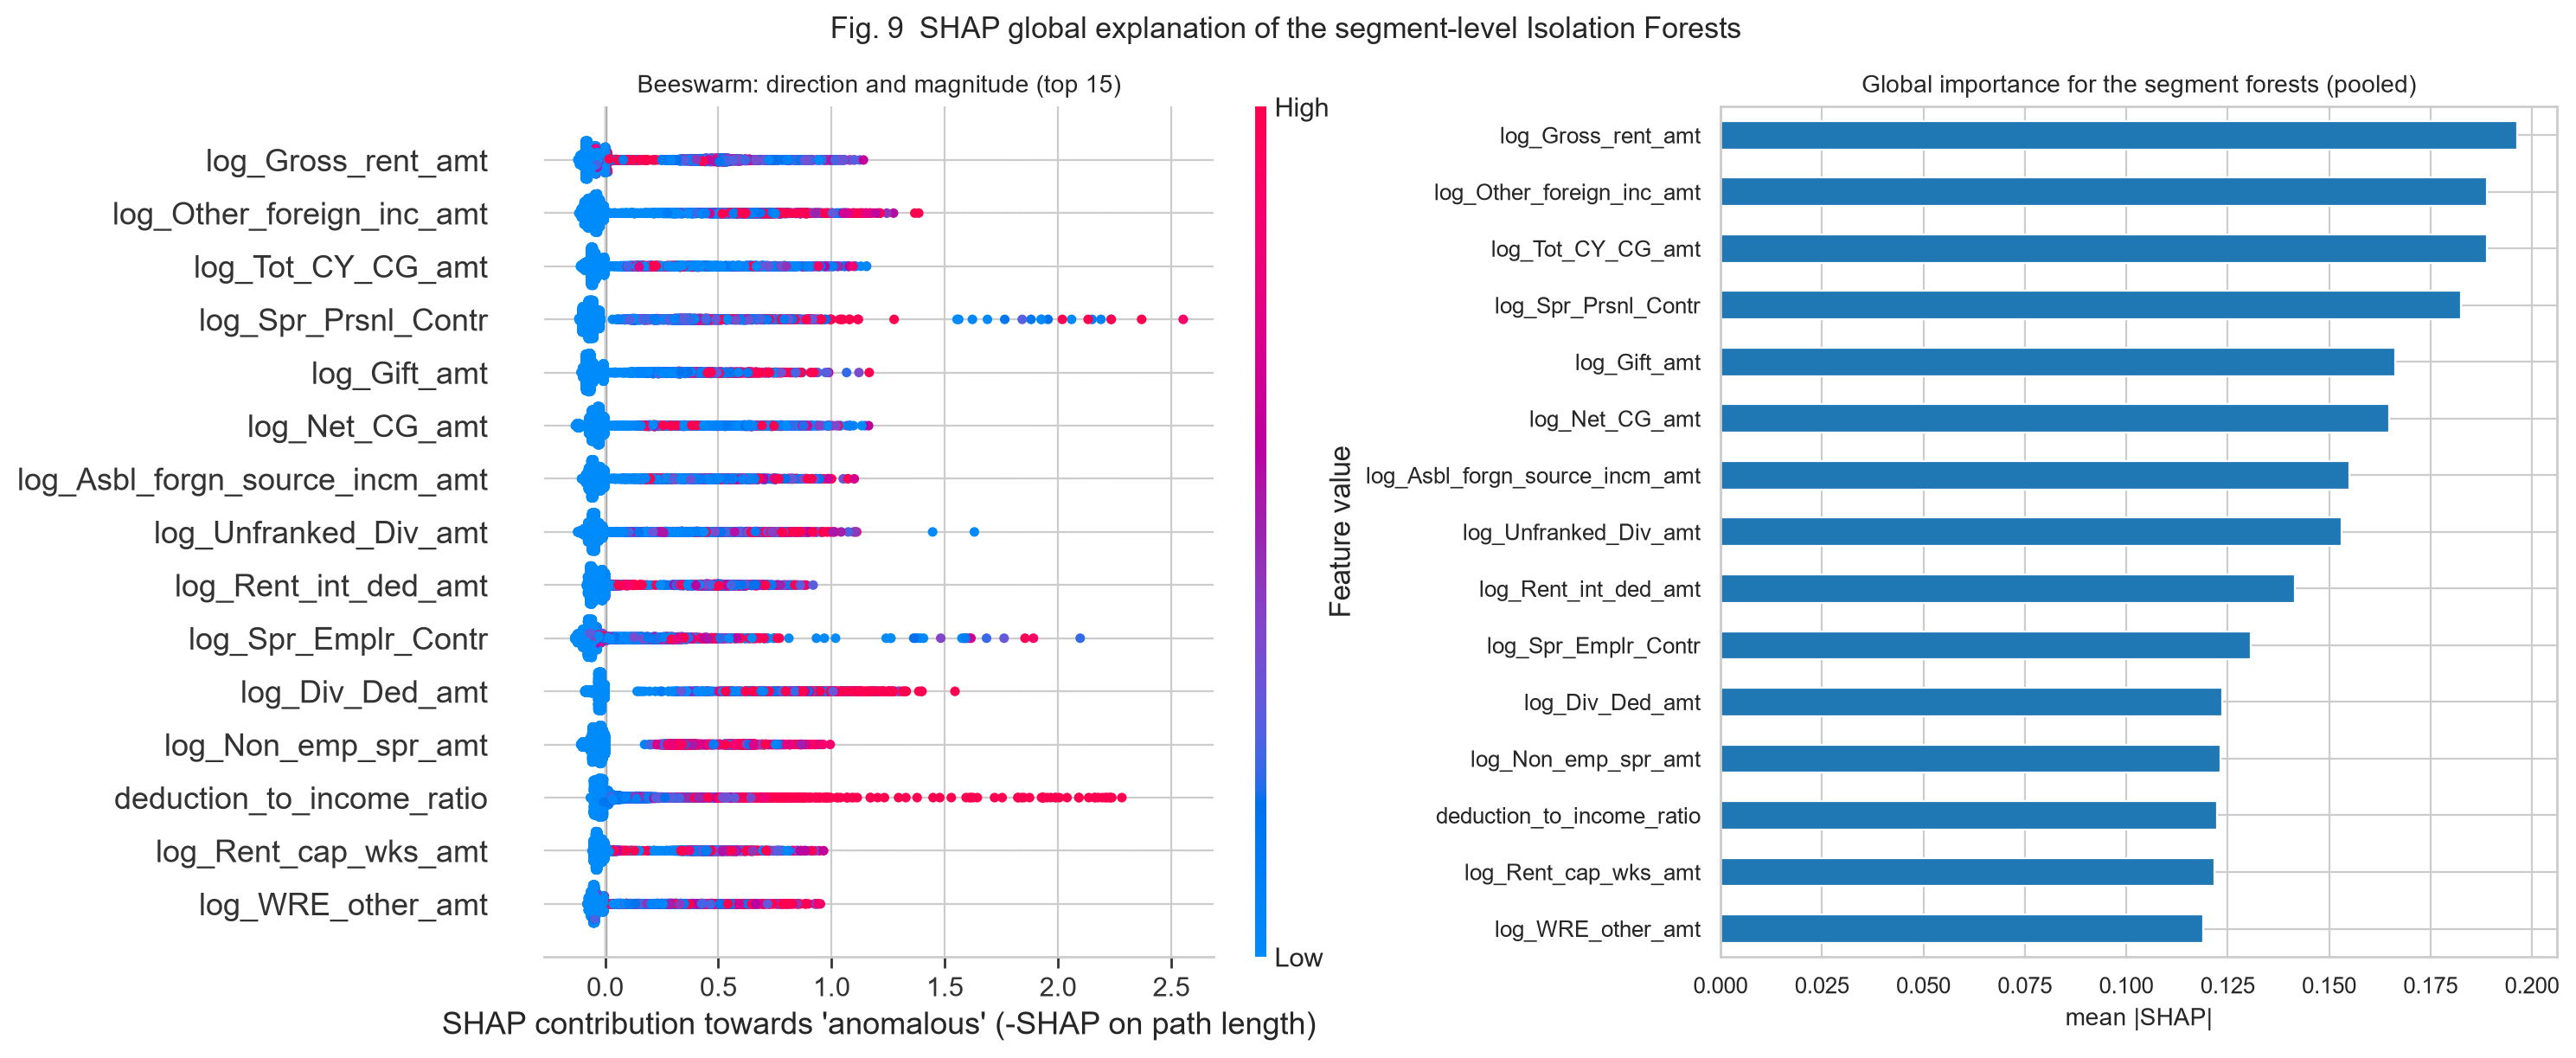
\includegraphics[width=\linewidth]{figures/fig09_shap_if_global.png}
    \caption{SHAP global explanation of the segment-level Isolation Forests.}
    \label{fig:shap_if_global}
\end{figure}

No single feature reaches a 50\% flag rate: even among the top 1\% of taxpayers on gross rent, capital gains or personal superannuation contributions only 15--27\% are flagged (Table~\ref{tab:flag_thresholds}). For rarely reported items the value at which the flag rate first reaches 10\% is simply the point at which the item becomes non-zero (other foreign income, unfranked dividends and capital gains: \$1--\$3), and a 25\% flag rate is reached only for other foreign income above \$380 and rental interest deductions above about \$59,000. The quantities that actually determine a flag are the within-segment score cut-offs of Table~\ref{tab:thresholds} (0.523--0.545); flags are multivariate, so a high value on one feature raises the chance of review but never decides it.

\begin{table}[H]
    \centering
    \caption{Empirical single-feature flag thresholds (pooled): the feature value above which the flag rate reaches 10\%, 25\% and 50\%, and the flag rate among the top 1\% of each feature.}
    \label{tab:flag_thresholds}
    \footnotesize
    \resizebox{\textwidth}{!}{%
    \begin{tabular}{lrrrrr}
        \toprule
        Feature & Value for flag rate $\geq$10\% & $\geq$25\% & $\geq$50\% & Flag rate in top 1\% (\%) & Feature p99 \\
        \midrule
        Gross\_rent\_amt & 6,833.6 & -- & -- & 18.2 & 58,116.8 \\
        Other\_foreign\_inc\_amt & 1.0 & 380.0 & -- & 26.9 & 1,710 \\
        Tot\_CY\_CG\_amt & 2.0 & -- & -- & 16.2 & 69,780.8 \\
        Spr\_Prsnl\_Contr & 548.0 & -- & -- & 17.4 & 59,355.8 \\
        Gift\_amt & 651.0 & -- & -- & 16.3 & 2,634.1 \\
        Net\_CG\_amt & 3.0 & -- & -- & 16.9 & 28,761.3 \\
        Asbl\_forgn\_source\_incm\_amt & 2.0 & -- & -- & 14.6 & 5,926.1 \\
        Unfranked\_Div\_amt & 2.0 & -- & -- & 19.3 & 1,117.1 \\
        Rent\_int\_ded\_amt & 164.7 & 59,227.6 & -- & 19.8 & 31,072.3 \\
        Spr\_Emplr\_Contr & 19,260.2 & -- & -- & 16.1 & 30,573.3 \\
        \bottomrule
    \end{tabular}}
\end{table}

Fig.~\ref{fig:shap_local} gives waterfall explanations for three flagged taxpayers. (a) The highest-ranked injected record, a wage earner into which inflated rental deductions were injected, was isolated mainly by items that were unusual before injection: personal superannuation contributions at 3.3 times income, dividend deductions of \$127,766, capital gains and a cost of managing tax affairs equal to income; the injected rental item (capital-works deductions of \$102,713) appears only ninth, which shows why the primary forests recover injected ratio anomalies poorly. (b) The highest-ranked natural profile is a landlord with foreign income, gifts exceeding income, a net capital gain of \$84,172 and deductions 3.3 times income, the lawful-but-rare profile that dominates the review list. (c) The borderline record, a wage earner exactly at the 2\% cut-off, is isolated by a termination payment of \$28,116 and other income of \$101,728 alongside small dividend items, each contributing modestly. Each explanation is a statement about the model, that these reported amounts and ratios are what isolated the record from its peers, and directs an officer to the items worth checking.

\begin{figure}[H]
    \centering
    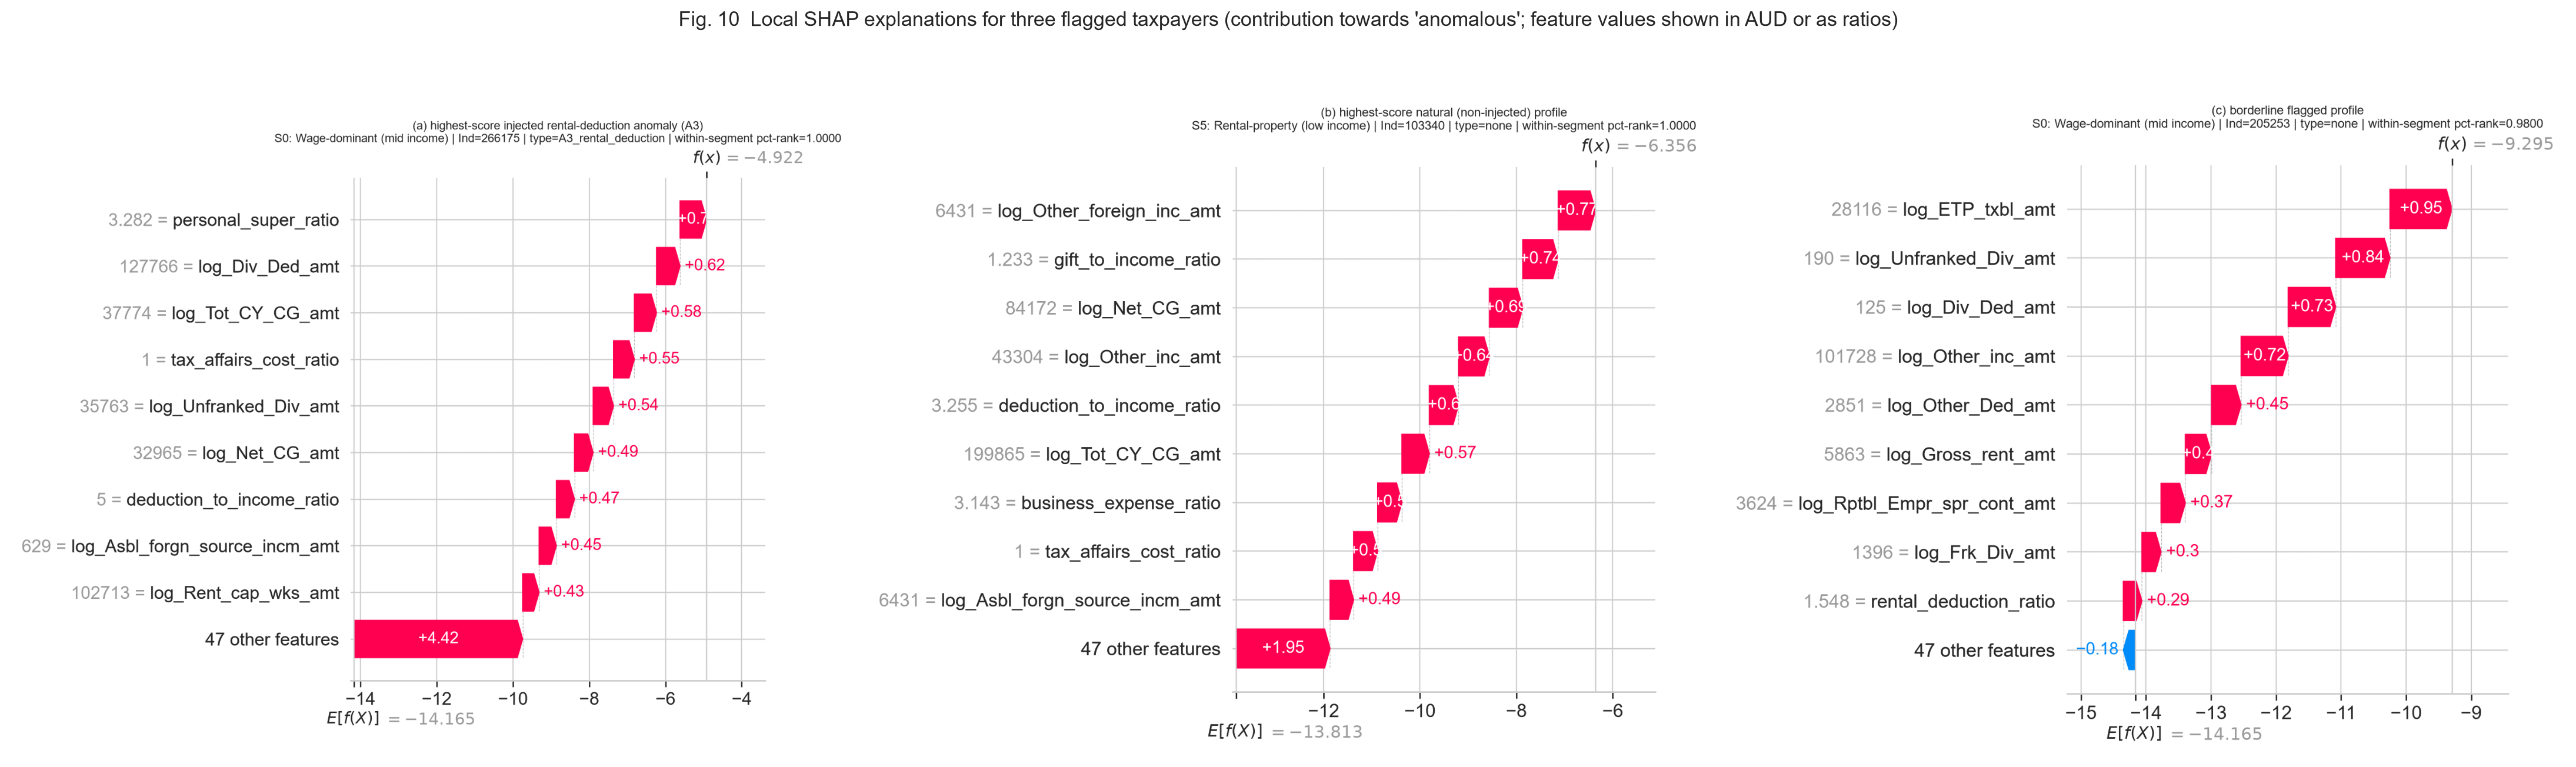
\includegraphics[width=\linewidth]{figures/fig10_shap_local_waterfalls.png}
    \caption{Local SHAP explanations for three flagged taxpayers (contribution towards ``anomalous'').}
    \label{fig:shap_local}
\end{figure}

For the Random Forest (Fig.~\ref{fig:shap_rf}) the taxable-income ratio dominated (mean $|$SHAP$|$ 0.095), followed by the deduction-to-income, rental-deduction and business-expense ratios (0.048, 0.035, 0.028), exactly the quantities the injection mechanisms perturbed. The rank correlation between the Random Forest and Isolation Forest importance orderings was $-0.07$: the models attend to different features because they were built for different tasks.

\begin{figure}[H]
    \centering
    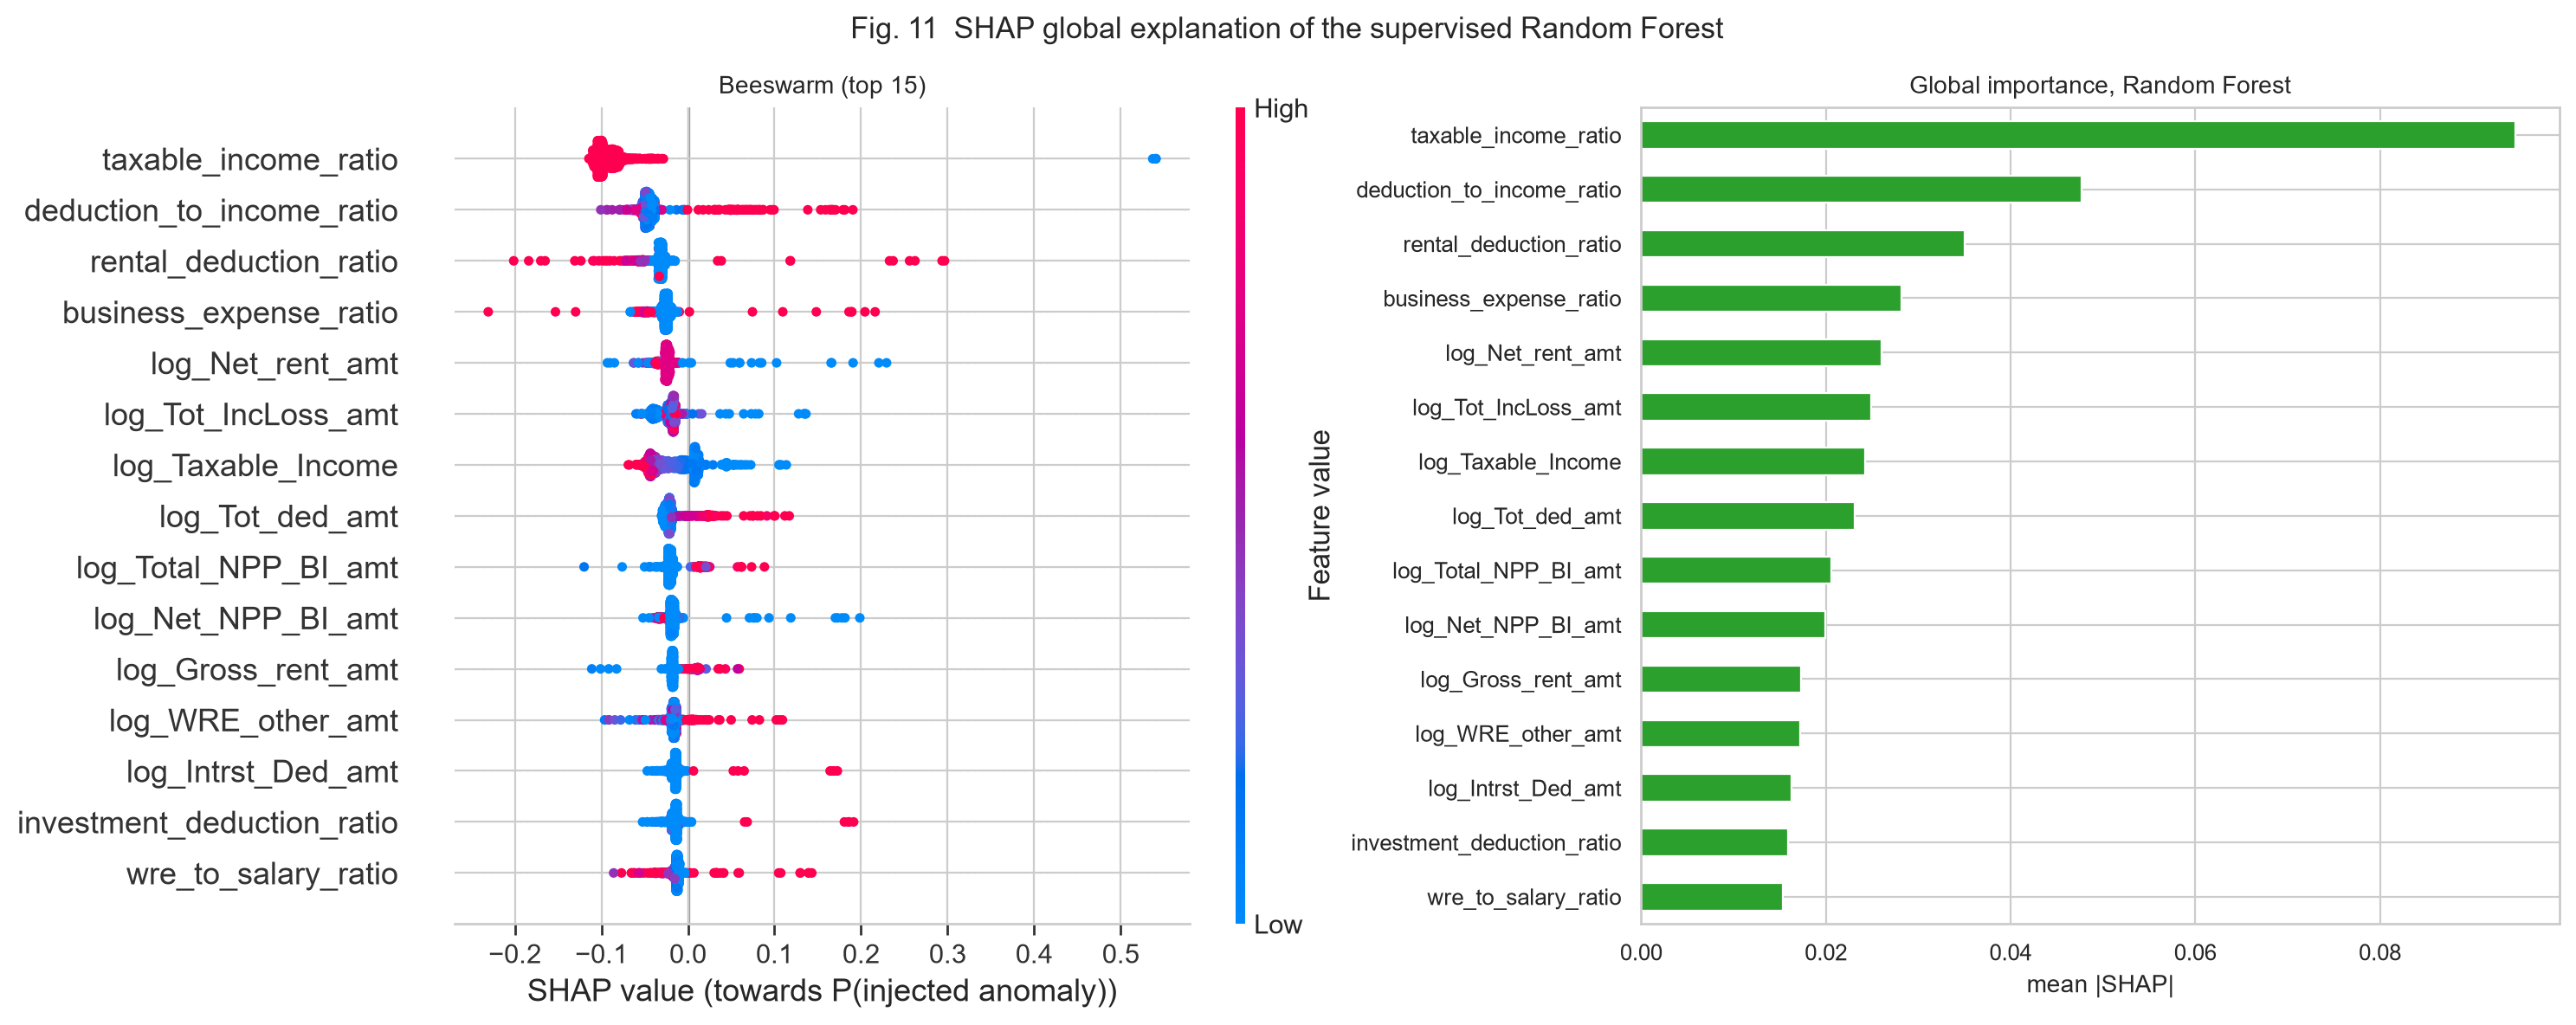
\includegraphics[width=\linewidth]{figures/fig11_shap_rf_global.png}
    \caption{SHAP global explanation of the supervised Random Forest.}
    \label{fig:shap_rf}
\end{figure}

In a compliance context the SHAP output says that a high deduction-to-income relationship, large rental interest deductions and large investment-type income contributed strongly to the segment forests' classification of a taxpayer as unusual, and that an internally inconsistent taxable income was the single most informative signal for the supervised model. None of this establishes that any taxpayer acted improperly; large capital gains or foreign income are lawful and common at the top of the income distribution.
